\documentclass[12pt]{article}
\usepackage{amsfonts}
\usepackage{fancyhdr}
\usepackage[a4paper, top=2.5cm, bottom=2.5cm, left=2.2cm, right=2.2cm]{geometry}
\usepackage{times}
\usepackage{amsmath}
\usepackage{changepage}
\usepackage{amssymb}
\usepackage{graphicx}%
\setcounter{MaxMatrixCols}{30}
\newtheorem{theorem}{Theorem}
\newtheorem{acknowledgement}[theorem]{Acknowledgement}
\newtheorem{algorithm}[theorem]{Algorithm}
\newtheorem{axiom}{Axiom}
\newtheorem{case}[theorem]{Case}
\newtheorem{claim}[theorem]{Claim}
\newtheorem{conclusion}[theorem]{Conclusion}
\newtheorem{condition}[theorem]{Condition}
\newtheorem{conjecture}[theorem]{Conjecture}
\newtheorem{corollary}[theorem]{Corollary}
\newtheorem{criterion}[theorem]{Criterion}
\newtheorem{definition}[theorem]{Definition}
\newtheorem{example}[theorem]{Example}
\newtheorem{exercise}[theorem]{Exercise}
\newtheorem{lemma}[theorem]{Lemma}
\newtheorem{notation}[theorem]{Notation}
\newtheorem{problem}[theorem]{Problem}
\newtheorem{proposition}[theorem]{Proposition}
\newtheorem{remark}[theorem]{Remark}
\newtheorem{solution}[theorem]{Solution}
\newtheorem{summary}[theorem]{Summary}
\usepackage{enumitem}
\usepackage[utf8]{inputenc}
\newenvironment{proof}[1][Proof]{\textbf{#1.} }{\ \rule{0.5em}{0.5em}}
\usepackage{tikz}
\usetikzlibrary{fit,arrows,calc,positioning}
\usepackage{graphicx}
\usepackage{wrapfig}
\usepackage{float}
\usepackage{datetime}
\newdateformat{specialdate}{\twodigit{\THEDAY}.\twodigit{\THEMONTH}.\THEYEAR}
\usepackage{amssymb}
\usepackage{ifsym}
\usepackage{mathtools}
\usepackage{listings}
\usepackage{lipsum}  

\newcommand{\blue}[1]{\color{blue}#1\color{black}}
\newcommand{\red}[1]{\color{red}#1\color{black}}
\newcommand{\green}[1]{\color{green}#1\color{black}}
\newcommand{\N}{\mathbb{N}}
\newcommand{\Q}{\mathbb{Q}}
\newcommand{\R}{\mathbb{R}}
\newcommand{\C}{\mathbb{C}}
\newcommand{\Z}{\mathbb{Z}}
\renewcommand\labelenumii{\theenumi.\arabic{enumii}.}
\newcommand{\code}[1]{\texttt{#1}}

\begin{document}
	
	\title{6. Exercise}
	\author{Timo Bergerbusch 344408 \\ Thomas Näveke 311392 \\ Shu Xing 381176}
	\date{\specialdate\today}
	\maketitle
	
	\section*{Exercise 6.1}
	\section*{Exercise 6.2 (Datalog)}
	\subsection*{6.2.1}
		\begin{enumerate}[label=\alph*)]
			\item \code{parent(X,Y) :- child (Y,X).}
			\item \code{married(X,Y) :- child(Z,X) , child(Z,Y).}
			\item \code{sister(X,Y) :- child(X,Z), child(Y,Z), NOT male(X).} \\
				Comment: assuming halfsisters are also considered sisters.
			\item \code{halfbrother(X,Y) :- parent(Z,X), parent(Z,Y), parent(N,X), NOT parent(N,Y), male(X).}\\
				Comment: assuming every person has only two parents.
		\end{enumerate}
	\subsection*{6.2.2}
		\begin{itemize}
			\item Datalog program 1: \\				
				\begin{figure}[H]
					\centering
					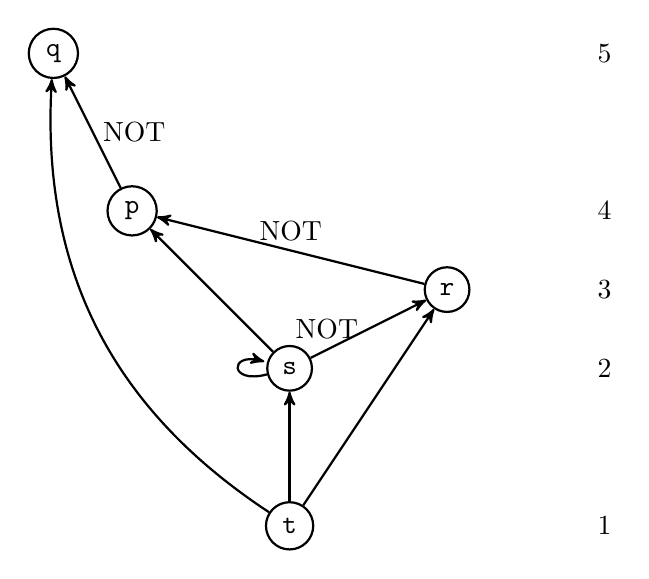
\begin{tikzpicture}[->,>=stealth',auto,node distance=3cm, thick]
					\node (5) at (9,4) {5};
					\node (4) at (9,2) {4};
					\node (3) at (9,1) {3};
					\node (2) at (9,0) {2};
					\node (1) at (9,-2) {1};
					
					\node[circle,draw] (q) at (2,4) {\code{q}};
					\node[circle,draw] (p) at (3,2) {\code{p}};
					\node[circle,draw] (s) at (5,0) {\code{s}};
					\node[circle,draw] (r) at (7,1) {\code{r}};
					\node[circle,draw] (t) at (5,-2) {\code{t}};
					
					\draw[thick] (p) edge node[right] {NOT} (q);
					\draw[thick, bend angle=30, bend left] (t) edge (q);
					
					\draw[thick] (s) edge (p);
					\draw[thick] (r) edge node[above] {NOT} (p);
					
					\path (s) edge[loop left] (s);
					\draw[thick] (t) edge (s);
					
					\draw[thick] (t) edge (r);
					\draw[thick] (s) edge node[left] {NOT} (r);
					\end{tikzpicture}
				\end{figure}
				No two predicates in a layer depend negatively on each other, so the program is stratified.
				
			\item Datalog program 2:\\
				\begin{figure}[H]
					\centering
					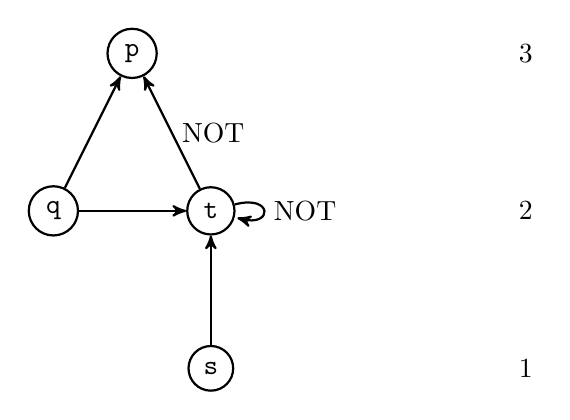
\begin{tikzpicture}[->,>=stealth',auto,node distance=3cm, thick]
					\node (3) at (6,4) {3};
					\node (2) at (6,2) {2};
					\node (1) at (6,0) {1};
					
					\node[circle, draw] (p) at (1,4) {\code{p}};
					\node[circle, draw] (q) at (0,2) {\code{q}};
					\node[circle, draw] (t) at (2,2) {\code{t}};
					\node[circle, draw] (s) at (2,0) {\code{s}};
					
					\draw[thick] (q) edge (p);
					\draw[thick] (t) edge node[right] {NOT} (p);
					
					\draw[thick] (q) edge (t);
					\draw[thick] (t) edge[loop right] node {NOT} (t);
					\draw[thick] (s) edge (t);
					\end{tikzpicture}
				\end{figure}
				Since the predicate \code{t} depends negatively on itself program 2 is not stratified
		\end{itemize}
\end{document}


















